%
% main.tex -- Paper zum Thema <relativ>
%
% (c) 2020 Autor, OST Ostschweizer Fachhochschule
%
% !TEX root = ../../buch.tex
% !TEX encoding = UTF-8
%
% git checkout dev -- sections images main.tex packages.tex references.bib Makefile Makefile.inc .gitignore
%

\chapter{Relativistische Mechanik\label{chapter:relativ}}
\kopflinks{Thema}
\begin{refsection}
\chapterauthor{Selvin Blöchlinger}

Das vorliegende Kapitel behandelt die Herleitung der Gesetze der relativistischen Mechanik
mithilfe der Variationsrechnung.
Es stützt sich grösstenteils auf~\cite{relativ:landau}.


\section{Das Relativitätsprinzip 
\label{relativ:section:relativistik}}
\rhead{Das Relativitätsprinzip}

Um relativistische Mechanik verstehen zu können,
muss natürlich zuerst auf das Relativitätsprinzip eingegangen werden.
Dabei gibt es zwei wesentliche Unterschiede zur klassischen Mechanik.

Der erste wichtige Unterschied ist, dass die Zeit unter relativistischer Betrachtung keine absolute Grösse ist.
Geschehenes kann also nicht einfach anhand eines starren Zeitstrahls erklärt werden, sondern die Zeit ist abhängig vom Betrachter.
Man geht über vom dreidimensionalen Raum in die vierdimensionale Raumzeit, in welcher die Welt relativistisch beschrieben wird.
Punkte in dieser Raumzeit werden als \emph{Ereignisse} oder \emph{Weltpunkte} bezeichnet.

Der zweite Unterschied ist,
dass die Geschwindigkeit der Wirkungsausbreitung begrenzt ist,
und zwar durch die Lichtgeschwindigkeit
\(c=\num{299792458}\unit[per-mode = fraction]{\metre\per\second}\).
Diese ist zwar auch in der klassischen Mechanik eine Konstante,
jedoch ist die Geschwindigkeit der Wirkungsausbreitung dort unbegrenzt.
Ein einfaches Beispiel, um dies zu veranschaulichen,
ist die Betrachtung von starren Körpern in der klassischen Mechanik.
Wird ein starrer Körper beispielsweise an einem Punkt angestossen,
so muss sich, gemäss Definition eines starren Körpers,
jeder Teil dieses Körpers augenblicklich und zeitgleich in Bewegung setzen.
Dies bedeutet also, dass sich die Wirkung (Anstossen des Körpers)
vom Punkt aus, in dem dieser angestossen wurde,
mit unendlicher Geschwindigkeit in alle Teile des Körpers ausbreitet.
Unter relativistischer Betrachtung ist dies also nicht möglich,
und es kann somit auch keine starren Körper geben.


\subsection{Der Abstand 
\label{relativ:section:abstand}}

Ebenfalls muss der Begriff des Abstands für die relativistische Mechanik umformuliert werden.
In der klassischen Mechanik ist der euklidische Abstand
\begin{equation}
    ds=\sqrt{dx^2 + dy^2 + dz^2}
    \label{relativ:eqn:abstand-klass}
\end{equation}
in den drei Raumkoordinaten \(x, y, z\)
für alle Bezugssysteme identisch.

Analog dazu gibt es in der relativistischen Mechanik den erweiterten Abstand
\begin{equation}
    ds = \sqrt{c^2dt^2 - dx^2 - dy^2 - dz^2}
    \label{relativ:eqn:abstand-relativ}
\end{equation}
in den Koordinaten \(ct, x, y, z\) der Raumzeit.
Dieser ist ebenfalls für verschiedene Bezugssysteme identisch.
Ausgehend von der Invarianz des Abstandes lassen sich
viele Gesetze der relativistischen Mechanik herleiten.


\subsection{Die Eigenzeit 
\label{relativ:section:eigenzeit}}

Angenommen, wir beobachten eine Uhr,
welche sich in unserem Koordinatensystem um die Strecke
\(\sqrt{dx^2 + dy^2 + dz^2}\)
bewegt.
Im Koordinatensystem der Uhr gilt
\(dx' = dy' = dz' = 0\).
Gemäss der Invarianz des Abstands gilt somit
\begin{equation*}
    \underbrace{ds^2 = c^2 dt^2 - dx^2 - dy^2 - dz^2}_{\text{Unser Koordinatensystem}}
        = \underbrace{ds'^2 = c^2 dt'^2}_{\text{Koordinatensystem der Uhr}} .
\end{equation*}
Wird dieser Ausdruck nach dem Differential der Zeit im System der Uhr aufgelöst,
so folgt
\begin{equation}
    dt' = \frac{ds}{c} = \frac{ds'}{c}
    = dt \sqrt{1 - \frac{dx^2+dy^2+dz^2}{c^2 dt^2}}
    = dt \sqrt{1 - \frac{v^2}{c^2}},
    \label{relativ:eqn:differential-eigenzeit}
\end{equation}
mit der Geschwindigkeit \(v\) der Uhr.
Dieses Zeitdifferential kann nun zur Zeitdifferenz
\begin{equation}
    t_2' - t_1' = \int_{t_1}^{t_2} dt \sqrt{1 - \frac{v^2}{c^2}}
    \label{relativ:eqn:eigenzeit}
\end{equation}
integriert werden.
Das ist nun die Zeit, die von der bewegten Uhr gemessen wird.
Eine solche Zeit, welche von einer Uhr,
die sich mit einem Gegenstand mitbewegt, gemessen wird,
nennt man \emph{Eigenzeit}.
Durch den Ausdruck unter der Wurzel wird klar,
dass die Zeitdifferenz \(t_2'- t_1'\) kleiner ist
als \(t_2 - t_1\) im Referenzsystem.
Daher kommt auch der Ausdruck
``bewegte Uhren gehen langsamer''.


\subsection{Koordinatentransformationen 
\label{relativ:section:koordtrafo}}

Koordinatentransformationen werden benutzt,
um Koordinaten aus einem Bezugssystem in diejenigen eines anderen Bezugssystems umzurechnen.
In der Physik dienen sie beispielsweise dazu,
ein System oder einen Vorgang aus einer anderen Perspektive bzw.
von einem anderen Referenzpunkt aus zu beschreiben.

\subsubsection{Galilei-Transformation 
\label{relativ:section:galilei-trafo}}

In der klassischen Mechanik gibt es die folgenden,
intuitiven Transformationen, um zwischen verschiedenen Bezugssystemen
zu vergleichen:
\[
\begin{aligned}
    &\text{Translation in der Zeit: } && t \rightarrow t + b \\
    &\text{Translation im Raum: } && \vec{r} \rightarrow \vec{r} + \vec{a} \\
    &\text{Orthogonale Drehung: } && \vec{r} \rightarrow A \vec{r} \\
    &\text{Transformation auf ein Bezugssystem mit Relativgeschwindigkeit: } && \vec{r} \rightarrow \vec{r} + \vec{v} \cdot t .
\end{aligned}
\]
Eine Kombination aus diesen Transformationen wird als Galilei-Transformation bezeichnet.
Ein einfaches Beispiel dafür ist in Abbildung~\ref{relativ:fig:galilei-trafo} zu finden.
\begin{figure}
    \centering
    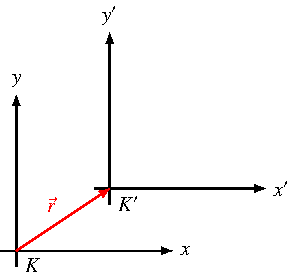
\includegraphics{papers/relativ/tikz/galilei_trafo.pdf}
    \caption{Darstellung einer einfachen Galilei-Transformation in \(\mathbb{R}^2\)
    vom Koordinatensystem \(K\) zum System \(K'\).
    Sie besteht lediglich aus einer Translation um den Vektor \(\vec{r}\).
    \label{relativ:fig:galilei-trafo}}
\end{figure}
Die Galilei-Transformation bildet die Grundlage für die Methoden der klassischen Mechanik,
wie beispielsweise die Addition von Kräftevektoren.

\subsubsection{Lorentz-Transformation 
\label{relativ:section:lorentz-trafo}}

In der relativistischen Mechanik und auch im Elektromagnetismus
muss man sich hingegen der Lorentz-Transformation bedienen.
Sie stellt eine Erweiterung der Galilei-Trans"-for"-ma"-tion dar,
die sich unter anderem aus der Invarianz des Abstands ergibt,
und kann wesentlich kompliziertere Formeln annehmen.

Als Beispiel sei hier die in Abbildung~\ref{relativ:fig:lorentz-trafo-koords}
dargestellte Situation gegeben, in welcher sich ein System \(K'\)
entlang der \(x\)-Achse mit der konstanten Geschwindigkeit \(V\)
relativ zu einem Bezugssystem \(K\) bewegt, gegeben.
\begin{figure}
    \centering
    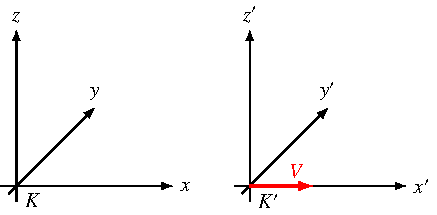
\includegraphics{papers/relativ/tikz/lorentz-trafo-koord.pdf}
    \caption{Bezugssystem \(K\) und ein zweites Koordinatensystem \(K'\),
    welches sich relativ zu \(K\) mit der konstanten Geschwindigkeit \(V\)
    entlang der \(x\)-Achse bewegt.
    \label{relativ:fig:lorentz-trafo-koords}}
\end{figure}
Für den Fall der klassischen Mechanik ist die Transformation einfach und
wir erhalten die Gleichungen
\begin{equation}
    t = t', \quad
    x = x' + Vt, \quad
    y = y', \quad \text{und} \quad
    z = z',
    \label{relativ:eqn:galilei-trafo-beisp}
\end{equation}
sofern man als Startzeitpunkt den Moment wählt,
in dem die beiden Koordinatensysteme am selben Ort sind.
Um den Erhalt des relativistischen Abstands zu gewährleisten,
ergeben sich jedoch (ohne Herleitung) die Gleichungen
\begin{equation}
    t = \frac{t' + \frac{V}{c^2}x'}{\sqrt{1-\frac{V^2}{c^2}}}, \quad
    x = \frac{x' + V t'}{\sqrt{1 - \frac{V^2}{c^2}}}, \quad
    y = y', \quad \text{und} \quad
    z = z'.
    \label{relativ:eqn:lorentz-trafo-beisp}
\end{equation}


\section{Relativistische Mechanik
\label{relativ:section:rel-mech}}
\rhead{Relativistische Mechanik}

\subsection{Elementarteilchen in der Relativitätstheorie
\label{relativ:section:elementarteilchen}}

Wie bereits in der Einleitung zu Abschnitt~\ref{relativ:section:relativistik} erwähnt,
kann es gemäss der Relativitätstheorie keine starren Körper geben.
Angemessener ist daher die Betrachtung \emph{punktförmiger Elementarteilchen}.
Der Zustand eines solchen Elementarteilchens ist dabei vollständig definiert durch
die drei Raumkoordinaten und die drei zugehörigen Geschwindigkeitskomponenten.


\subsection{Das Prinzip der kleinsten Wirkung
\label{relativ:section:kleinste-wirkung}}

Für die Berechnung der Bewegung von materiellen Teilchen geht man
von dem bereits in Kapitel~\ref{buch:chapter:mechanik} eingeführten
Maupertuisschen Prinzip der kleinsten Wirkung aus.
Dieses besagt, dass es für jedes mechanische System ein sogenanntes
Wirkungsintegral \(S\) gibt,
dass für diejenige Bewegung ein Minimum besitzt, die tatsächlich erfolgt.
Wie bereits zu erahnen ist, kann dieses Minimum durch die Variation \(dS\)
des Wirkungsintegrals ermittelt werden.

\subsubsection{Wirkungsintegral für ein freies Teilchen
\label{relativ:section:wirk-int-freies-teilchen}}

Nachfolgend wird das Wirkungsintegral und die Lagrange-Funktion
für ein freies Teilchen, das heisst ein Teilchen, welches nicht
unter dem Einfluss äusserer Kräfte oder Felder steht, hergeleitet.

Da dieses Integral unabhängig vom gewählten Koordinatensystem sein muss,
kann es nur von Skalaren und nicht von den Variablen \(x, y, z, t\) abhängen.
Das Wirkungsintegral hat daher die Form
\begin{equation}
    S = - \alpha \int_{a}^{b} ds,
\label{relativ:eqn:wirk-int-grundform}
\end{equation}
wobei \(\alpha\) eine vom Teilchen abhängige Konstante,
und \(a\) und \(b\) zwei Ereignisse in der Raumzeit sind.
Integriert wird über die Weltlinie des Teilchens,
d.h. entlang dessen Bahn durch die Raumzeit.

Das Wirkungsintegral lässt sich auch über die Zeit darstellen,
wobei es die Form
\begin{equation}
    S = \int_{t_1}^{t_2} L \, dt
\label{relativ:eqn:wirk-int-zeit}
\end{equation}
annimmt, mit der Lagrange-Funktion \(L\).
Ersetzt man \(ds\) in \eqref{relativ:eqn:wirk-int-grundform}
gemäss \eqref{relativ:eqn:differential-eigenzeit} und passt
die Integrationsgrenzen an, so erhält man
\begin{equation}
    S = -\int_{t_1}^{t_2} \alpha c \sqrt{1-\frac{v^2}{c^2}} dt
    \quad \text{und somit} \quad
    L = -\alpha c \sqrt{1-\frac{v^2}{c^2}}.
    \label{relativ:eq:wirk-int-lagrange}
\end{equation}

Zur Bestimmung der Teilchenkonstante \(\alpha\) beginnt man mit der Forderung,
dass die Lagrange-Funktion im Grenzfall \(c\rightarrow\infty\) in den
Ausdruck \(L=mv^2/2\) der klassischen Mechanik übergehen soll.
Mittels der Potenzreihe
\begin{equation*}
    \sqrt{1+w} = 1 + \frac{1}{2} w - \frac{1}{2\cdot4} w^2 +
    \frac{1\cdot3}{2\cdot4\cdot6} w^3 \mp \cdots, \quad
    -1\leq w \leq1
\end{equation*}
kann die Lagrange-Funktion aus
\eqref{relativ:eq:wirk-int-lagrange} beim Weglassen der
Glieder höherer Ordnung und mit der Substitution
\(w=-\frac{v^2}{c^2}\) entwickelt werden zu
\begin{equation}
    L = - \alpha c \sqrt{1-\frac{v^2}{c^2}}
    \approx -\alpha c \biggl(1 - \frac{v^2}{2c^2}\biggr)
    = -\alpha c + \frac{\alpha v^2}{2c}.
\end{equation}
Da Konstanten in der Lagrange-Funktion keinen Einfluss auf die Bewegungsgleichung haben,
kann der erste Term ignoriert werden. Somit bleibt die Forderung
\begin{equation}
    \frac{\alpha v^2}{2c} = \frac{mv^2}{2}
    \quad \text{und daraus ergibt sich} \quad
    \alpha = mc.
\end{equation}
Ein freies Teilchen besitzt folglich die Lagrange-Funktion
\begin{equation}
    L = -mc^2 \sqrt{1-\frac{v^2}{c^2}}.
\label{relativ:eqn:lagrange-freies-teilchen}
\end{equation}

\subsubsection{Wirkungsintegral für ein Teilchen im elektromagnetischen Feld
\label{relativ:section:wirk-int-em-feld}}

Das Wirkungsintegral für ein Elementarteilchen im elektromagnetischen Feld ist
\begin{equation}
    S = \int_a^b \biggl(-mc\,ds + \frac{e}{c} \bm{A}\,d\bm{r} - e\varphi\,dt\biggr)
    \label{relativ:eqn:wirk-int-em-feld}
\end{equation}
und somit eine Erweiterung von \eqref{relativ:eqn:wirk-int-grundform}.
Dabei ist \(\bm{A}\) das \emph{Vektorpotential des Feldes}\footnote{
    Auch bekannt als \emph{magnetisches Vektorpotential}.}
und \(\varphi\) das \emph{skalare Potential des Feldes}\footnote{
    Auch bekannt als \emph{elektrisches Potential}.}.
In der relativistischen Raumzeit schreibt man diese zwei Grössen
auch als Vierervektor \(A^i = (\varphi, \bm{A})\),
wobei \(\varphi\) zur Zeitkoordinate \(t\) gehört und
\(\bm{A}\) zu den räumlichen Koordinaten \(x, y, z\).
Als Integral über die Zeit geschrieben wird das Wirkungsintegral zu
\begin{equation}
    S = \int_{t_1}^{t_2} \biggl( -mc^2 \sqrt{1-\frac{v^2}{c^2}} + \frac{e}{c} \bm{A} \bm{v} - e \varphi \biggr) \, dt,
    \label{relativ:eqn:wirk-int-em-feld-zeit}
\end{equation}
wobei \(\displaystyle \bm{v} = \frac{d\bm{r}}{dt}\) der Geschwindigkeitsvektor der drei räumlichen Dimensionen ist.
Der Integrand in \eqref{relativ:eqn:wirk-int-em-feld-zeit} ist gerade die Lagrange-Funktion
\begin{equation}
    L = -mc^2 \sqrt{1-\frac{v^2}{c^2}} + \frac{e}{c} \bm{A} \bm{v} - e \varphi.
    \label{relativ:eqn:lagrange-em-feld}
\end{equation}


\section{Ladungen im Elektromagnetischen Feld
\label{relativ:section:em_feld}}
\rhead{Ladungen im Elektromagnetischen Feld}


\subsection{Elementarteilchen in der Relativitätstheorie
\label{relativ:section:elementarteilchen}}

Wie bereits in der Einleitung zu Abschnitt~\ref{relativ:section:relativistik} erwähnt,
kann es gemäss der Relativitätstheorie keine starren Körper geben.
Angemessener ist daher die Betrachtung \emph{punktförmiger Elementarteilchen}.
Der Zustand eines solchen Elementarteilchens ist dabei vollständig definiert durch
die drei Raumkoordinaten und die drei zugehörigen Geschwindigkeitskomponenten.


\subsection{Wirkungsintegral
\label{relativ:section:wirkungsintegral}}

Das Wirkungsintegral für ein Elementarteilchen im elektromagnetischen Feld ist
\begin{equation}
    S = \int_a^b \left(-mc\,ds + \frac{e}{c} \mathbf{A}\,d\mathbf{r} - e\varphi\,dt\right).
    \label{relativ:eqn:wirk-int-em-feld}
\end{equation}
Dabei ist \(A\) das \emph{Vektorpotential des Feldes}\footnote{
    Auch bekannt als \emph{magnetisches Vektorpotential}.}
und \(\varphi\) das \emph{skalare potential des Feldes}\footnote{
    Auch bekannt als \emph{elektrisches Potential}.}.
In der relativistischen Raumzeit schreibt man diese zwei Grössen
auch als Vierervektor \(A^i = (\varphi, \mathbf{A})\),
wobei \(\varphi\) zur Zeitkoordinate \(t\) gehört und
\(\mathbf{A}\) zu den räumlichen Koordinaten \(x, y, z\).
Als Integral über die Zeit geschrieben ergibt sich das Wirkungsintegral als
\begin{equation}
    S = \int_{t_1}^{t_2} \biggl( -mc^2 \sqrt{1-\frac{v^2}{c^2}} + \frac{e}{c} \mathbf{A} \mathbf{v} - e \varphi \biggr) \, dt,
    \label{relativ:eqn:wirk-int-em-feld-zeit}
\end{equation}
wobei \(\displaystyle \mathbf{v} = \frac{d\mathbf{r}}{dt}\) der Geschwindigkeitsvektor der drei räumlichen Dimensionen ist.
Der Integrand in \eqref{relativ:eqn:wirk-int-em-feld-zeit} ist gerade die Lagrange-Funktion
\begin{equation}
    L = -mc^2 \sqrt{1-\frac{v^2}{c^2}} + \frac{e}{c} \mathbf{A} \mathbf{v} - e \varphi
    \label{relativ:eqn:lagrange-em-feld}
\end{equation}


\subsection{Bewegungsgleichung
\label{relativ:section:bewegungsgleichung}}

Bei der Berechnung der Bahn eines Elementarteilchens
in einem elektromagnetischen Feld geht man von
der vereinfachenden aber angemessenen Annahme aus,
dass die Rückwirkung des Teilchens auf das Feld vernachlässigt werden kann
\footnote{Konkret muss für diese Annahme beispielsweise
für die magnetische Feldstärke
\(H \ll \frac{m^2c^4}{e^3}\) erfüllt sein.
Die rechte Seite ergibt dabei für ein Elektron
eine magnetische Feldstärke von
\(\frac{m_e^2c^4}{e^3} \approx
\frac{(\qty{9e-31}{\kilogram})^2 (\qty{3e8}{\metre\per\second})^4}{(\qty{1.6e-19}{\ampere\second})^3}
\approx \qty[per-mode=fraction]{1.6e30}{\ampere\per\metre}\),
was im Vakuum einer magnetischen Flussdichte von
\(\mu_0 \cdot \qty[per-mode=fraction]{1.6e30}{\ampere\per\metre} \approx
\qty[per-mode=fraction]{1.25e-6}{\tesla\metre\per\ampere} \cdot
\qty[per-mode=fraction]{1.6e30}{\ampere\per\metre} =
\qty{2e24}{\tesla}\)
entspricht, einem Wert weitaus grösser als alle bekannten physikalischen Phänomene.}.

Die Bewegungsgleichung ergibt sich aus der Variation des Wirkungsintegrals
mit der Euler-Lagrange-Differentialgleichung
\begin{equation}
    \frac{d}{dt} \frac{\partial L}{\partial \mathbf{v}} - \frac{\partial L}{\partial \mathbf{r}} = 0,
    \label{realtiv:eqn:euler-lagrange-em-feld}
\end{equation}
wobei \(L\) in \eqref{relativ:eqn:lagrange-em-feld} gegeben ist.
Die Ableitung nach dem Geschwindigkeitsvektor \(\mathbf{v}\) ergibt
\begin{equation}
    \frac{\partial L}{\partial \mathbf{v}} =
    mc^2 \frac{-\frac{2}{c^2}\mathbf{v}}{-2\sqrt{1-\frac{v^2}{c^2}}}
    + \frac{e}{c} \mathbf{A} - 0
    = \frac{m \mathbf{v}}{\sqrt{1-\frac{v^2}{c^2}}} + \frac{e}{c} \mathbf{A}.
    \label{realtiv:eqn:part-diff-v}
\end{equation}
Dies wird auch als verallgemeinerter Teilchenimpuls \(\mathbf{P}\) bezeichnet,
wovon der linke Term der gewöhnliche (relativistische) Impuls \(\mathbf{p}\)
des Teilchens ist.

Die partielle Ableitung von \(L\) nach \(\mathbf{r}\) ergibt dann
\begin{equation}
    \frac{\partial L}{\partial \mathbf{r}} = \nabla L
    = 0 + \frac{e}{c} \operatorname{grad} \mathbf{Av} - e \operatorname{grad} \varphi.
    \label{realtiv:eqn:part-diff-r}
\end{equation}
Wir können nun \eqref{realtiv:eqn:part-diff-v} und \eqref{realtiv:eqn:part-diff-r}
in \eqref{realtiv:eqn:euler-lagrange-em-feld} einsetzen und erhalten
\begin{equation}
    \frac{d}{dt} \biggl(\mathbf{p} + \frac{e}{c} \mathbf{A}\biggr)
    - \frac{e}{c} \operatorname{grad} \mathbf{Av} + e \operatorname{grad} \varphi = 0.
    \label{realtiv:eqn:euler-lagrange-em-eingesetzt}
\end{equation}
Diese Differentialgleichung kann mittels Formeln der Vektoranalysis
umgeformt werden, um schliesslich
\begin{equation}
    \frac{d\mathbf{p}}{dt} = -\frac{e}{c} \frac{\partial\mathbf{A}}{\partial t}
    - e \operatorname{grad} \varphi +
    \frac{e}{c} \mathbf{v} \times \operatorname{rot} \mathbf{A}
    \label{realtiv:eqn:euler-lagrange-em-eingesetzt}
\end{equation}
zu erhalten.

\begin{beispiel}
\label{realtiv:bsp:teilchen-konst-e-feld}
Gehen wir von der einfachen Situation aus,
in der sich ein Elektron durch ein statisches
elektrisches Feld bewegt und \(\mathbf{A}\)
somit dem Nullvektor entspricht.
Der Geschwindigkeitsvektor des Elektrons sei
\(\mathbf{v}_0 = \mathbf{v}(t=0) =(\beta c, 0, 0)^T\), wobei
\(\beta \in (0, 1)\).
Die Differentialgleichung reduziert sich somit zu
\begin{equation}
    \frac{d\mathbf{p}}{dt} =
    \frac{m_e}{\sqrt{1-\frac{v^2}{c^2}}} \frac{d\mathbf{v}}{dt} =
    - e \operatorname{grad} \varphi,
    \label{relativ:eqn:euler-lagrange-bsp-1}
\end{equation}
mit der Elektronenmasse \(m_e\) und der Elementarladung \(e\).
Die Ableitung des Impulses entspricht somit lediglich
dem Gradienten des elektrischen Potentials, oder dem elektrischen Feld.
Der wesentliche Unterschied zur klassischen Mechanik ist hierbei
der bekannte relativistische Korrekturfaktor
\(\sqrt{1-\frac{v^2}{c^2}}\).

Nehmen wir nun beispielsweise an,
dass das elektrische Feld lediglich eine \(x\)-Komponente hat,
sprich \( \operatorname{grad} \varphi = (E_x, 0, 0)^T \),
so ergibt sich für die Ableitung des Geschwindigkeitsvektors
\begin{equation}
    \frac{d}{dt}
        \begin{pmatrix}
            v_x \\
            v_y \\
            v_z
        \end{pmatrix} =
        - \frac{e \sqrt{1-\frac{v^2}{c^2}}}{m_e}
        \begin{pmatrix}
            E_x \\
            0 \\
            0
        \end{pmatrix}.
    \label{relativ:eqn:bsp-abl-v-vec}
\end{equation}
Hierbei ist klar, dass sich die Geschwindigkeitskomponenten
in \(y\)- und \(z\)-Richtung nicht ändern können.
Zusammen mit der Anfangsgeschwindigkeit \(\mathbf{v}_0\)
ergibt sich somit die nichtlineare Differentialgleichung erster Ordnung
\begin{equation}
    \frac{d}{dt} v_x = - \frac{e E_x}{m_e} \sqrt{1-\frac{v_x^2}{c^2}}
\end{equation}
für die Geschwindigkeit in \(x\)-Richtung \(v_x\).
Mittels Separierung erhält man die Lösung
\begin{equation}
    v_x(t) = c \operatorname{sin} \biggl(
        \frac{k_1 - \frac{e}{m_e}t}{c}
    \biggr)
\end{equation}
mit der zu bestimmenden Konstanten \(k_1\).
\todo{Dies kann kaum stimmen?!}
% Zum Zeitpunkt \(t=0\) erhält man
% \begin{equation}
%     v_x(0) = c \operatorname{sin} \biggl(\frac{k_1}{c}\biggr)
%     = \beta c \Leftrightarrow
%     k_1 = c \operatorname{arcsin}(\beta)
% \end{equation}

\end{beispiel}



\printbibliography[heading=subbibliography]
\end{refsection}
